\lstnewenvironment{Code03_03}[1][]{\lstset{basicstyle=\small\ttfamily, columns=fullflexible,framexrightmargin=+.1\textwidth, keywordstyle=\color{red}\bfseries, commentstyle=\color{blue},language=C++, basicstyle=\small, numbers=left, numberstyle=\tiny, stepnumber=1, numbersep=5pt, frame=shadowbox, #1}}{}

\chapter{Classi per la gestione dell'intersezione}

Nel modello che abbiamo preso in considerazione noi le fratture hanno una rappresentazione in $\mathbb{R}$ e, nel caso della \textit{Biforcazione}, hanno un unico punto in comune. 
Nella rappresentazione 2D, invece, la regione in comune è un triangolo. \\

\begin{figure}[htbp]
\centering
\includegraphics[scale=.5]{img/subcap3_3/TriangoloBiforcazione.eps}
%\includegraphics[width=0.65\textwidth]{img/TriangoloBiforcazione.eps}
\caption{Struttura della biforcazione 2D}\label{Biforcazione}
\end{figure}

Il nostro modello trascura ovviamente delle informazioni, ma nel caso di fratture con uno spessore sufficientemente piccolo rispetto a quelle del dominio, può essere considerato una buona approssimazione della realtà.\\

Per ricavare le condizioni d'interfaccia nel caso della biforcazione per modello ridotto passiamo per la rappresentazione in $\mathbb{R}^{2}$.
Nel caso 2D le fratture hanno uno spessore e possiamo delimitare un triangolo di intersezione unendo i punti di incontro dei loro bordi. \\
Presi \textbf{N} il vettore delle normali ai lati del triangolo, \textbf{$K_{I}$} la matrice di permeabilit\`{a} all'intersezione e una costante \textit{t} possiamo definire:
\begin{center}
	$ S = \textit{t} \, diag( \textbf{N}$ \textbf{$K_{I}$} $ \textbf{N}^{T} ) $
\end{center}
Definite ora \textbf{C} matrice dei vettori che uniscono il baricentro, punto C, del triangolo con il punto medio  di ogni lato e \textbf{$P_{c}$} matrice di proiezione sullo spazio nullo della matrice di base per \textbf{C}, possiamo trovare la matrice di trasmissibilit\`{a}:
\begin{center}
	$ T = \frac{1}{\textbf{I}}( \textbf{N}$ \textbf{$K_{I}$} $ \textbf{N}^{T} ) + $\textbf{$P_{c}$} $\textbf{S}$\textbf{$P_{c}$}
\end{center}
%\textbf{u} = \left\lbrace \u_{0}, \u_{1}, \u_{2} \right\rbrace
%$\textbf{\pi} = \left\lbrace \pi_{0}, \pi_{1}, \pi_{2} \right\rbrace $
Le variabili con cui ci troviamo a lavorare sono:
	\begin{enumerate}
	\item[-] \textbf{u} : vettore dei flussi
	\item[-] $p_{I}$ :  pressione nel punto di intersezione delle assi delle tre fratture;
	\item[-] \textbf{$\pi$}: vettore delle pressioni nel punto di incontro fra l'asse della frattura i-esima con un lato del triangolo;
	\end{enumerate} 
e le condizioni che dobbiamo porre all'intersezione sono:
\begin{center}			
	$\left \{
		\begin{array}{l}	
	 		\textbf{u} - p_{I}T\textbf{1}_{3}+T\Pi=0  \\ \\
     	 	\sum_{k=0}^2 u_{k} = p_{I} - \pi  \\
		\end{array}
	\right.$
\end{center} \label{condizioniinterfaccia}

\noindent  Queste sono le condizioni d'interfaccia che verranno imposte nel punto di intersezione delle fratture.\\ 
\par In questa parte di codice per gestire sia il calcolo delle matrici introdotte precedentemente, che i punti e la geometria del triangolo di intersezione, abbiamo usato la libreria matematica \textit{Eigen}.\\
\par Note le basi teoriche possiamo passare a descrivere le principali classi del codice che definiscono la struttura e le propriet\`{a} della biforcazione in uno spazio bidimensionale.

\newpage
\begin{figure}[htbp]
\centering
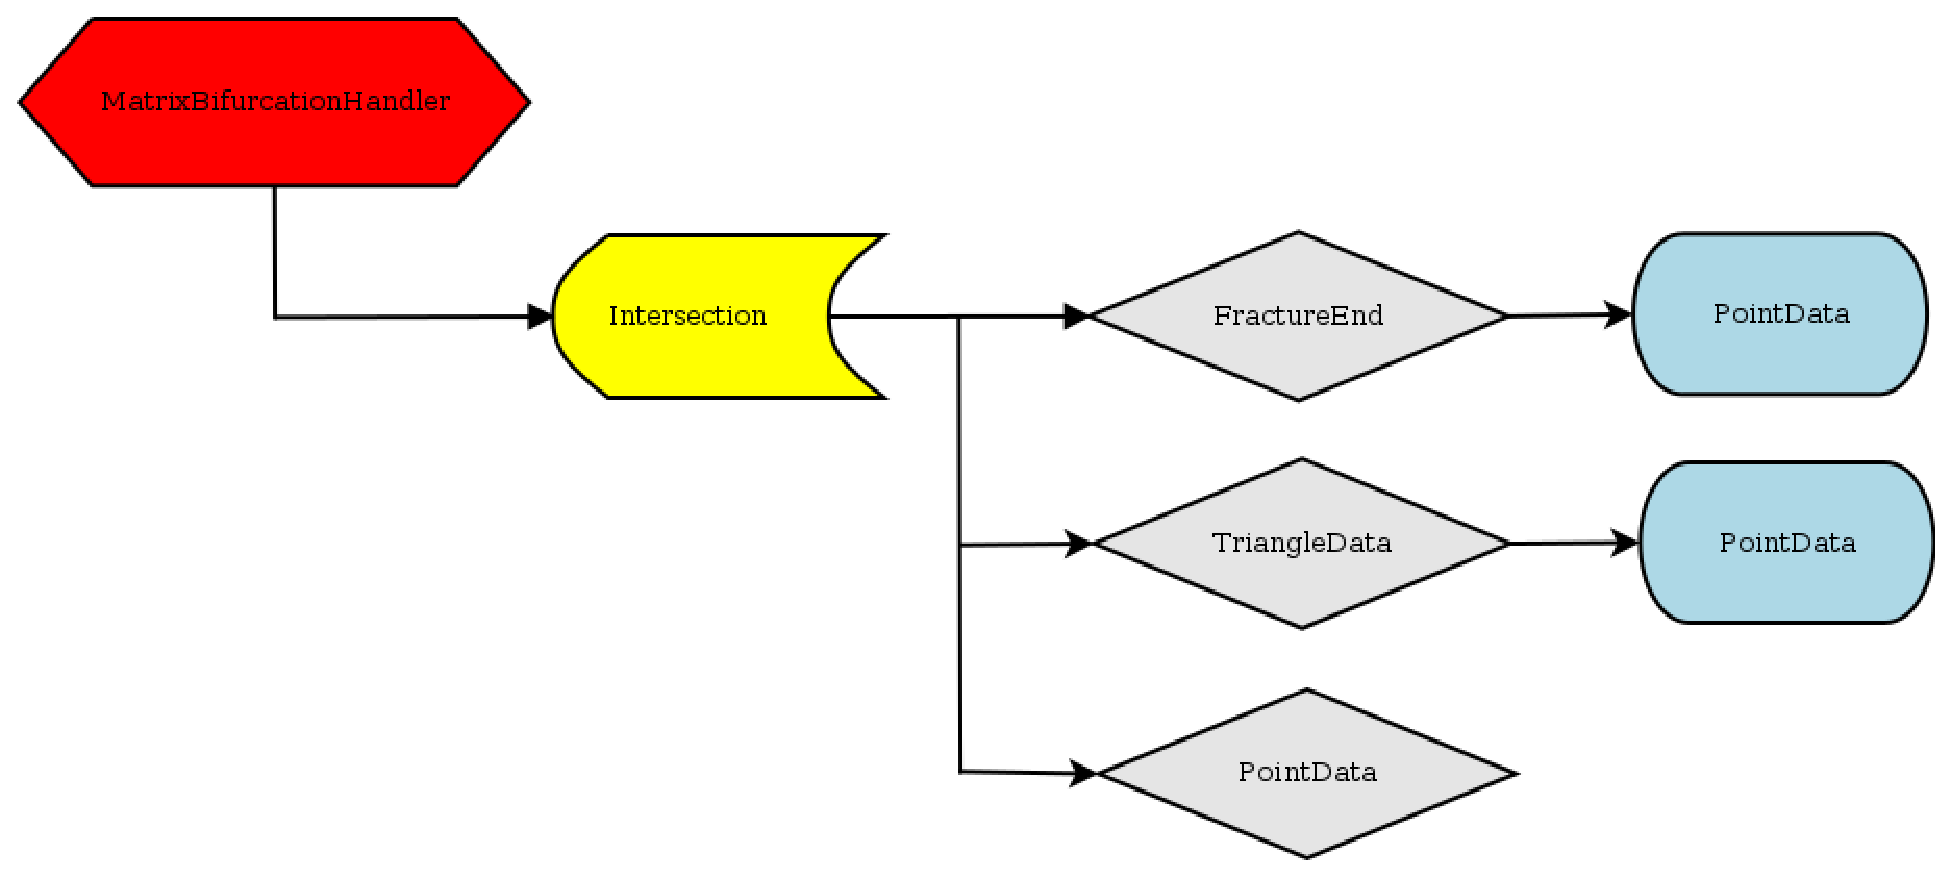
\includegraphics[height=7cm, width=1\textwidth]{img/subcap3_3/MatrixBifurcationHandler2.eps}
\caption{Inclusione tra le varie classi che costituiscono il triangolo di intersezione}\label{Inclusione classi MatrixBifurcationHandler}
\end{figure}

\section{La Classe \texttt{MatrixBifurcationHandler}}
La classe \texttt{MatrixBifurcationHandler} contiene le matrici associate a una biforcazione e implementa i metodi per calcolarle.  Il fine ultimo è il calcolo della matrice di trasmissibilità T.

\noindent I campi fondamentali della classe sono:
	\begin{enumerate}
	\item[-] \texttt{M\_intersection}: di tipo Intersection, contiene tutte le informazioni base per poter ricavare le matrici;
	\item[-] \texttt{M\_T}: matrice T di trasmissibilità necessaria per l'imposizione delle condizioni di interfaccia.
	\end{enumerate} 
\begin{Code03_03}[caption={Classe \texttt{Intersection}}]
class MatrixBifurcationHandler
{
 public:
	MatrixBifurcationHandler( const GetPot& dataFile,
				const std::string& section = "mediumData/",
				const std::string& subsection = "darcy/");
	
	void setMatrices ( FracturePtrContainer_Type& fractures );
	
	[ ... ]
	
	void computeT( scalar_type t=6.0 );

	[ ... ]

 private:

	Matrix2d M_K;
	Intersection_Type M_intersection;
	Matrix32 M_N;
	Matrix32 M_C;
	Matrix32 M_Qc;
	Matrix3d M_Pc;
	Matrix3d M_T;
};
\end{Code03_03}

\section{La Classe \texttt{Intersection}}

La class \texttt{Intersection}, definita in \texttt{Geometry.h}, contiene tutte le informazioni relative ad una biforcazione in uno spazio 2D necessarie per il calcolo delle matrici associate al triangolo di intersezione.
I campi fondamentali della classe sono:
	\begin{enumerate}
	\item[-] \texttt{M\_intersection}: di tipo PointData, rappresenta il punto di intersezione;
	\item[-] \texttt{M\_tangents}: vettore contenente le tangenti alle fratture coinvolte;
	\item[-] \texttt{M\_normals}: vettore contenente le normali alle fratture coinvolte;
	\item[-] \texttt{M\_intersectionTriangle}:di tipo TriangleData, rappresenta il triangolo di intersezione, i cui vertici sono i punti d'incontro dei bordi delle fratture.
	\end{enumerate} 

\begin{Code03_03}[caption={Classe \texttt{Intersection}}]
class Intersection
{
 public:
	[ ... ]
	
	void setIntersection( FracturePtrContainer_Type& M_FracturesSet );
	
	[ ... ]
 private:
	
	[ ... ]	
	
	PointData M_intersection;
	
	Vector2d M_tangents [ 3 ];
	Vector2d M_normals [ 3 ];
	
	TriangleData M_intersectionTriangle;
};	
\end{Code03_03}

\section{Classe \texttt{PointData} e Classe \texttt{TriangleData}}
Queste classi rappresentano un punto e un triangolo come grandezze geometriche.
Il punto geometricamente viene rappresentato come una grandezza zero dimensionale con due variabili, una \textit{x} e una \textit{y}.
Un triangolo è invece  rappresentato geometricamente dai punti che lo costituiscono.\\
\noindent La classe \texttt{PointData} ci permette di definire un punto e di poterlo manipolare con le operazioni di somma, differenza e prodotto.\\
\noindent La classe \texttt{TriangleData} ci permette di definire un triangolo e di calcolarne l'area. Inoltre sono stati implementati i metodi necessari per la costruzione del triangolo di intersezione.
